\documentclass[conference]{IEEEtran}
\usepackage{graphicx}
\usepackage[T1]{fontenc}
\usepackage{mathptmx}
\usepackage{booktabs}
\usepackage{amsmath}
\usepackage{url}
\usepackage[hidelinks]{hyperref}
\graphicspath{{../../results/}}
\title{Roomors: Hotel Booking Analytics and Cancellation Risk Prioritization}
\author{\IEEEauthorblockN{Job Russel Enriquez and John Cyruz Patron}\IEEEauthorblockA{BSIT--401I, Group 4.2\\Foundations of Business Analytics\\Jose Rizal University}}
\begin{document}
\maketitle
\begin{abstract}
Booking cancellations complicate reservation planning because recorded demand does not always become a completed stay. This study develops a local decision-support dashboard and evaluates cancellation classifiers using the Hotel Booking Demand dataset. The original 119,390 records are analyzed alongside an 87,396-record exact-deduplicated sample consistent with the group's earlier exploratory notebook. Descriptive analysis finds a 27.49\% cancellation rate in this sample, with higher rates at City Hotel and among online travel agency bookings. A Streamlit application presents five headline indicators, six descriptive visuals, and hotel, market-segment, and arrival-date filters. Predictive analysis compares a majority-class baseline, logistic regression, and a random forest using chronological booking-date partitions and exclusion of unresolved earlier labels. Logistic regression is selected on validation average precision. On 17,561 later test bookings, it achieves ROC-AUC of 0.7180, average precision of 0.4694, and F1 of 0.3078 at a fixed 0.50 threshold. Its highest-risk decile contains 977 cancellations among 1,757 bookings, yielding 2.01-fold enrichment over the test cancellation rate. Results support a limited confirmation-priority prototype, while temporal degradation, deduplication assumptions, snapshot features, and arrival-window truncation prevent claims of proven cancellation reduction or revenue improvement.
\end{abstract}
\begin{IEEEkeywords}
hotel bookings, cancellation prediction, descriptive analytics, dashboard, chronological evaluation
\end{IEEEkeywords}

\section{Introduction}
A hotel reservation is an expression of planned demand rather than a guaranteed completed stay. When reservations are canceled, managers may need to revise room availability, staffing expectations, and confirmation activity. A large raw cancellation count is difficult to interpret without the size of the booking group from which it comes. A manager therefore needs both a descriptive view of exposure and an operationally meaningful way to prioritize limited follow-up capacity.

This project asks: how can reservation and revenue managers identify booking groups with elevated cancellation risk and prioritize confirmation before arrival? The intended users are managers of the two properties represented in the supplied data. The decisions supported are which hotel and channel combinations merit investigation, which advance-booking groups need attention, and which reservations should enter a capacity-limited follow-up queue. The prototype does not make pricing decisions, revoke valid reservations, or prescribe overbooking levels.

The project contributes three connected artifacts. First, it translates an earlier exploratory notebook into a reproducible descriptive analysis with explicit denominators. Second, it implements a local interactive dashboard with five indicators, six descriptive charts, and three filters. Third, it evaluates two predictive models against a majority baseline under chronological separation. These artifacts are packaged for local execution and GitHub version control; no cloud deployment or external API is required.

\section{Related Work}
Antonio, de Almeida, and Nunes published the underlying hotel booking demand data for research and education \cite{dataset}. Their description identifies a resort and a city property, arrival coverage from July 2015 through August 2017, and removal of identifying hotel and customer information. This establishes the unit of analysis and geographic scope, but does not make the observations representative of the entire hospitality industry.

Earlier work by the same authors treats cancellation prediction as a classification problem relevant to hotel demand management \cite{hotelprediction}. That work motivates a connection between risk estimation and reservation decisions. Its reported performance cannot be used as a target that this project has achieved: features, sample composition, temporal setup, and operational availability can differ. Our study emphasizes a reproducible local application and a conservative evaluation of later bookings.

Random forests combine randomized tree predictors \cite{breiman}; they offer a useful nonlinear comparison to logistic regression. We test whether this flexibility improves validation ranking rather than assuming that a more complex model must be preferable. Scikit-learn supplies the implementations and composition tools used in this study \cite{sklearn}. Its common-pitfalls guidance supports fitting preprocessing on training data and consistently applying that fitted transformation to held-out data \cite{pitfalls}.

Saito and Rehmsmeier discuss why precision-recall analysis provides information that ROC analysis alone may obscure under class imbalance \cite{saito}. Consequently, we use validation average precision for model selection and report ROC-AUC, precision, recall, F1, and confusion counts as complementary measures. The metrics documentation further distinguishes prediction quality from subsequent decisions \cite{metrics}. This supports evaluating a fixed classification threshold separately from a staff-capacity ranking rule.

\section{Data and Exploratory Analysis}
\subsection{Source, Scope, and Preprocessing}
The supplied \texttt{hotel\_bookings.csv} contains 119,390 rows and 32 columns. It is the combined public dataset attributed to Antonio et al. \cite{dataset}, obtained through the Kaggle source documented in the earlier notebook. A row represents a recorded reservation; \texttt{is\_canceled} is the binary outcome. Important descriptive fields include hotel, lead time, arrival details, market segment, daily rate, stay length, and guest composition.

To reproduce Part A, exact duplicate rows are removed, leaving 87,396 records. Descriptive totals are calculated before model-specific exclusions. The final analytical CSV retains original missing values where appropriate so that model imputation can be learned from training data only. This differs from the earlier notebook's global fills while preserving its principal EDA counts. Arrival date is constructed from year, month, and day; total nights is the sum of weekday and weekend nights. Booking creation date is inferred as arrival date minus lead time.

Exact deduplication is an assumption, not proof of duplicate reservation identity. No unique booking identifier is supplied. The overall cancellation rate changes from 37.04\% on raw records to 27.49\% after deduplication. We therefore report a sensitivity analysis that retains the raw records. Neither sample should be described as an unbiased estimate of all hotel demand without qualification.

\subsection{Findings Summary}
Table~\ref{tab:eda} summarizes core evidence. Across the deduplicated sample, 24,025 reservations are canceled and 63,371 are not. City Hotel contributes 61.13\% of all records and has a higher within-hotel cancellation rate than Resort Hotel. Hotel-level comparison is necessary because unequal group sizes can dominate pooled totals.

\begin{table}[htbp]
\caption{Descriptive cancellation evidence, deduplicated sample}
\label{tab:eda}\centering\footnotesize
\begin{tabular}{lrrr}\toprule
Group & Bookings & Canceled & Rate (\%)\\\midrule
All records & 87,396 & 24,025 & 27.49\\
City Hotel & 53,428 & 16,049 & 30.04\\
Resort Hotel & 33,968 & 7,976 & 23.48\\
Online TA & 51,618 & 18,245 & 35.35\\
Direct & 11,804 & 1,737 & 14.72\\
Corporate & 4,212 & 510 & 12.11\\\bottomrule
\end{tabular}
\end{table}

Online TA combines substantial volume with a high cancellation share: 51,618 records, 59.06\% of the sample, and 35.35\% canceled. The Undefined segment has two canceled records out of two. Its 100\% rate is reported in a separate small-sample table rather than dominating the main segment chart. Groups with fewer than 30 selected records are separated by a transparent display rule, not removed from the KPIs. A small denominator does not support a broad policy conclusion.

Lead-time groups show an ordered descriptive pattern: cancellation is 8.43\% for 0--7 days, 25.37\% for 8--30 days, 32.01\% for 31--90 days, 34.98\% for 91--180 days, 39.68\% for 181--365 days, and 40.89\% beyond 365 days. The final group contains only 565 records. Pearson correlation between lead time and cancellation is approximately 0.185, so lead time alone is insufficient to reliably separate outcomes.

\begin{figure}[htbp]\centering
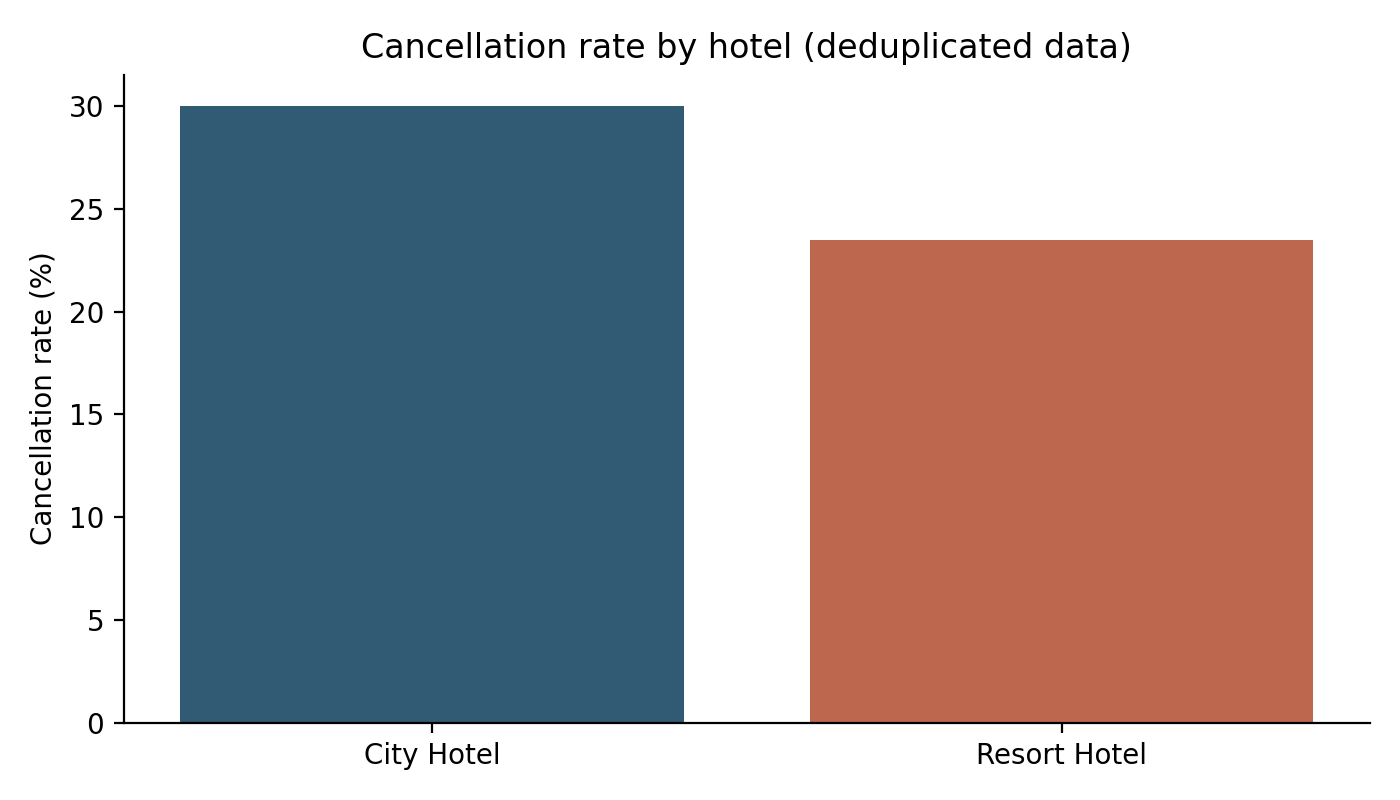
\includegraphics[width=\columnwidth]{hotel_rates.png}
\caption{Within-hotel cancellation rates in the 87,396-record sample. Group counts are unequal; the comparison describes association.}\label{fig:hotel}
\end{figure}

Booking notice is skewed: mean lead time is 79.89 days versus a median of 49, with quartiles at 11 and 125. Daily rate has mean 106.34, median 98.10, and quartiles at 72 and 134. Its minimum is -6.38 and maximum is 5,400 in dataset units. These values justify median summaries and investigation of extremes, not automatic deletion or treatment as verified revenue.

August has the largest pooled arrival count, 11,257, followed by July with 10,057. However, July and August appear in three observed years while the other months appear in two. The application therefore uses a chronological year-month series. Recorded arrivals are not room occupancy; neither complete inventory nor realized revenue is measured by booking counts alone.

\begin{figure}[htbp]\centering
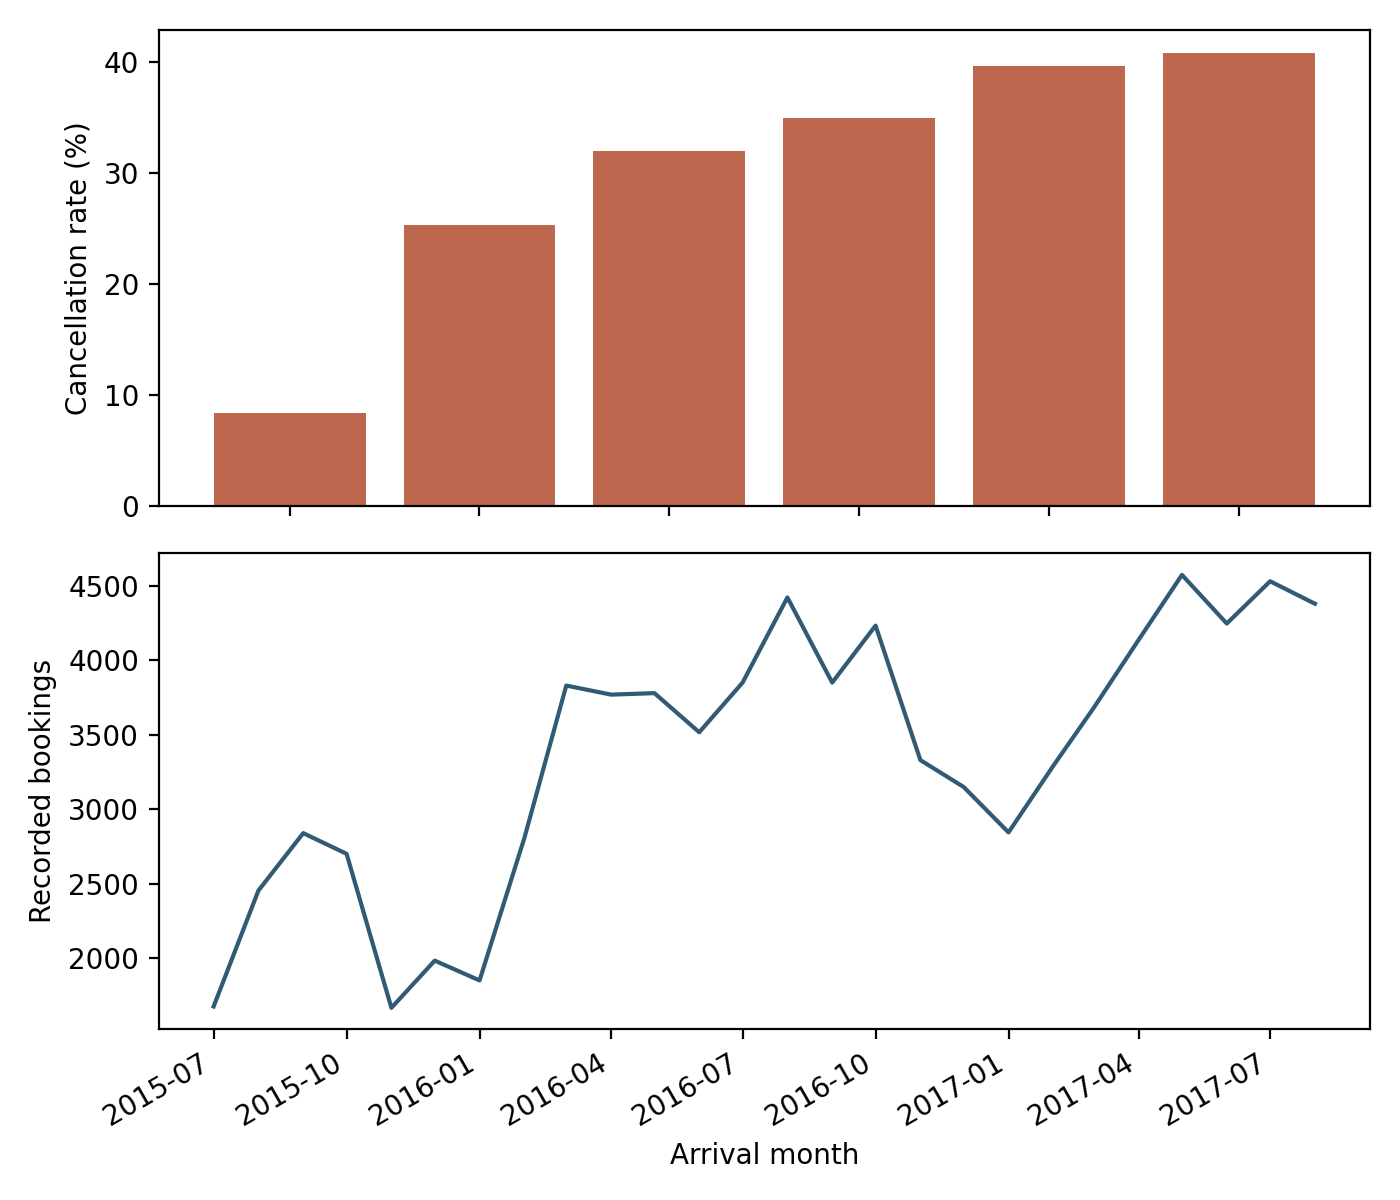
\includegraphics[width=\columnwidth]{eda_patterns.png}
\caption{Cancellation rates by lead-time group and recorded arrivals by chronological month. Counts reflect partial boundary years, not occupancy.}\label{fig:eda}
\end{figure}

\section{Dashboard Design and Insights}
\subsection{Audience and Information Architecture}
The dashboard serves reservation and revenue managers. Its opening sentence states the task: understand cancellation exposure and prioritize follow-up. The primary page contains five KPIs: total records, canceled records, cancellation rate, median lead time, and median daily rate. Counts show workload, the rate normalizes outcomes by group size, and the medians describe typical values despite skewness. Each KPI recalculates using the current descriptive filters.

The sidebar offers a hotel selector, a market-segment checkbox list with All and Clear controls, and an arrival-date range. A reset action restores the full sample. Three tabs separate Overview, Model performance, and Follow-up queue. This prevents retrospective group exploration from being mistaken for a change in the model evaluation sample. The model tab explicitly states that its metrics remain fixed when sidebar filters change. Interactive ROC and precision-recall curves display the selected model, with the original three-model comparison retained as an alternative view. Plain-language confusion counts explain missed cancellations and false flags.

\subsection{Visual Questions and Decisions}
The six descriptive visuals answer distinct questions. A hotel bar chart compares cancellation rates by property. A horizontal segment chart compares channel-associated exposure and includes booking counts in hover details. A chronological line chart shows recorded arrival volume, with cancellation rates in hover details. A lead-time bar chart supports advance-notice review. A rate box plot compares typical price distributions between hotels. Finally, a month-by-hotel heatmap locates periods whose cancellation rates deserve investigation; hover details include group counts. Segment hover details add descriptive 95\% Wilson intervals, which do not remove selection bias or dependence among bookings.

The rate box plot shows nonnegative values through the selected sample's 99th percentile for legibility. This display restriction does not delete rows from the KPIs or numerical summaries. Its note reports the number hidden. The heatmap leaves missing hotel-month combinations blank rather than implying a zero cancellation rate. Each chart has a concise conclusion and a business implication, with small-sample or coverage warnings where relevant.

The dashboard uses a restrained navy-and-blue palette on neutral surfaces, rounded panels, and a compact segmented navigation bar. System sans-serif typography supports reading, while monospaced KPI numerals support scanning. Chart titles state the questions directly, axis labels identify units, and whitespace separates content. Hover counts and downloadable filtered records provide detail without crowding every mark. Empty filter results display a message instead of generating a misleading empty dashboard.

\begin{figure*}[t]\centering
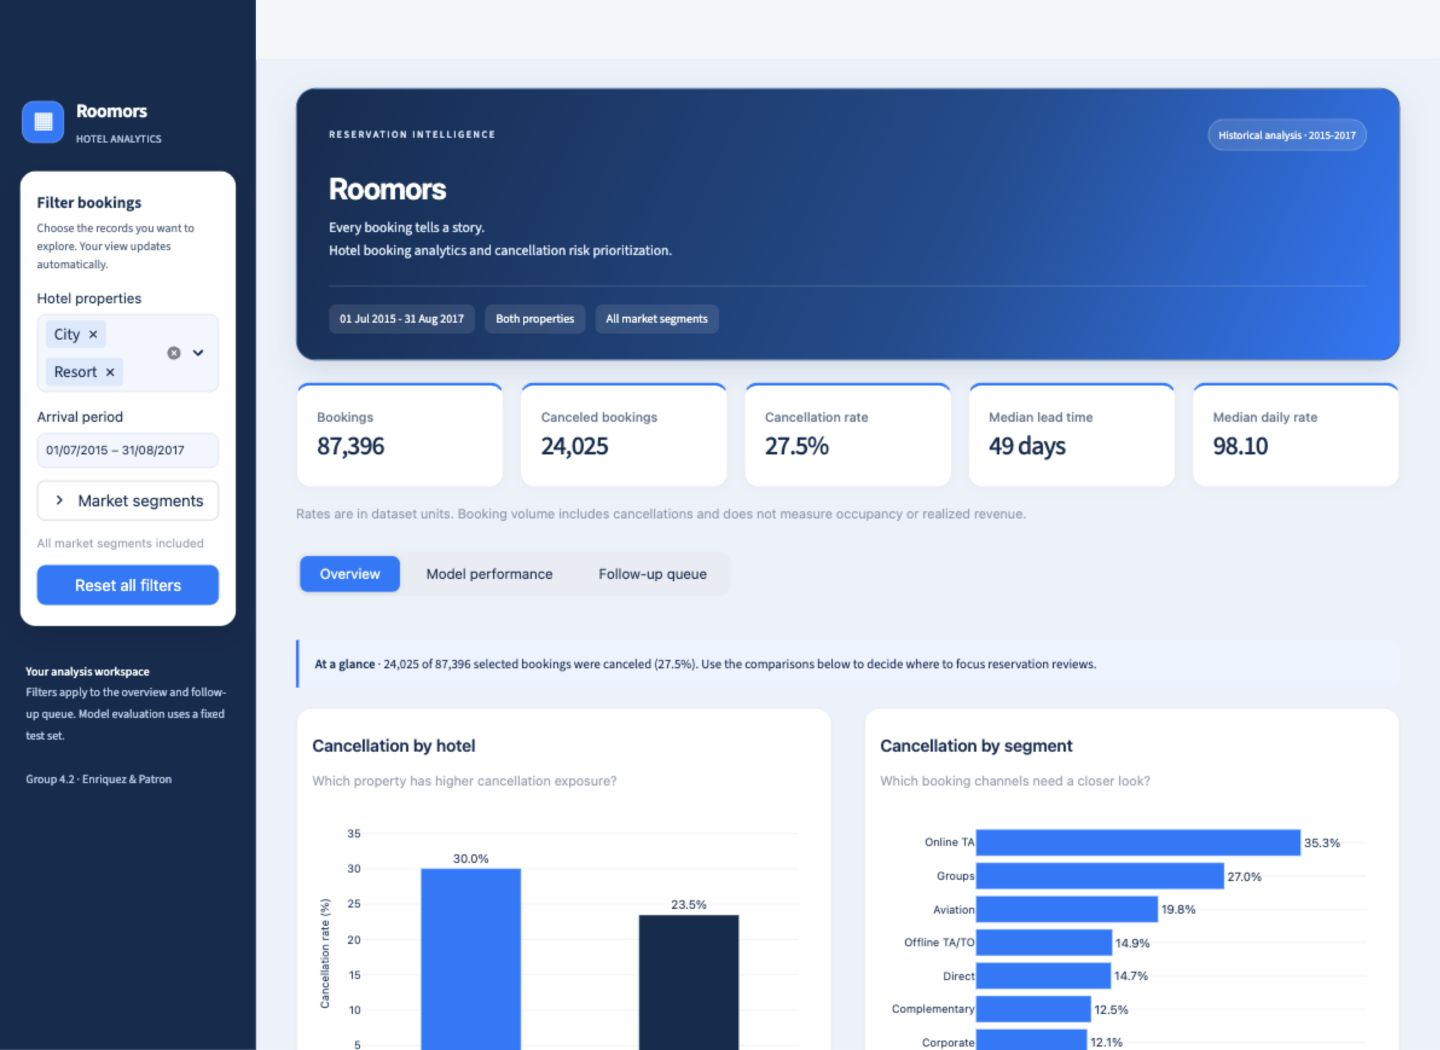
\includegraphics[width=0.74\textwidth]{dashboard.png}
\caption{Screenshot of the local dashboard. The overview links KPIs to booking comparisons; the sidebar supplies hotel, segment, and date filters.}\label{fig:dashboard}
\end{figure*}

\subsection{Local Execution and Verification}
The application is implemented with Streamlit and Plotly. Prepared CSVs and evaluation results are included, so users can open the app without retraining. A requirements file records package versions. The repository can be stored on GitHub and cloned to another computer, but execution occurs in the user's local Python process. GitHub Pages does not execute this application.

Verification checks the full-sample totals, a Resort-Hotel-only selection, and an empty hotel selection using Streamlit's application testing interface. The Resort Hotel selection returns 33,968 records, consistent with the exported summary. Browser inspection confirms that the chart views render. These checks establish basic functioning, not a formal usability study with hotel employees.

\section{Predictive Methodology}
\subsection{Target and Candidate Features}
The target is cancellation, with class one representing \texttt{is\_canceled=1}. Fifteen candidate booking-time fields are retained: lead time; arrival month and day; weekday and weekend nights; adults, children, and babies; hotel; meal; market segment; distribution channel; reserved room type; customer type; and country. They describe timing, planned stay, party composition, and booking context, and connect to the EDA patterns.

Final reservation status and its date are excluded from predictors because they reveal the outcome. Assigned room, booking changes, deposit type, daily rate, agency identifiers, prior-history measures, parking, and special requests are also excluded to reduce ambiguity about later updates and availability. Country is used only as a prototype context variable; it is not a justification for unequal service, penalties, or automatic rejection. A future pilot should assess group errors and consider removing it.

The source contains snapshots rather than a full event history. Even retained fields may have changed after booking. We therefore describe them as candidate booking-time fields, not verified historical features as of creation. Chronological splitting and excluding outcome columns reduce some leakage risks but do not eliminate this limitation.

\subsection{Chronological Partition and Label Availability}
Reservations are ordered by inferred creation date. The 60th and 80th percentile dates define September 21, 2016 and January 28, 2017 as validation and test origins. Same-date records stay together. Training uses bookings before the first origin, validation uses the interval between origins, and test uses later bookings.

A further purge requires training outcomes to be resolved before validation begins and validation outcomes to be resolved before test begins. Resolution is identified using reservation-status date for filtering only; it never enters the feature matrix. This excludes 6,851 otherwise eligible training rows and 7,632 validation rows. The usable sets contain 45,428 training, 9,924 validation, and 17,561 test bookings. Cancellation prevalence is respectively 27.64\%, 36.79\%, and 27.70\%.

This procedure emulates labels available at a scoring origin more conservatively than a random split. However, the dataset itself is truncated by arrival dates: future arrivals outside August 2017 are absent. A booking-created cohort is therefore not a complete live stream of all bookings known at that time. Purging unresolved labels can also alter the training mix. These constraints limit prospective interpretation.

\subsection{Preprocessing and Models}
Numerical inputs use training-median imputation and standard scaling. Categorical inputs use training-mode imputation and one-hot encoding with unknown categories ignored. A column transformer and pipeline keep these operations inside the fitted estimator, consistent with leakage-prevention guidance \cite{pitfalls}. The globally scaled columns from the earlier EDA notebook are not reused.

The majority baseline always predicts the training majority class. Logistic regression uses L2 regularization with $C=1$, maximum 1,200 iterations, and random seed 42. The random forest uses 160 trees, maximum depth 14, minimum 15 samples per leaf, square-root feature sampling, and seed 42. No synthetic balancing or test-driven hyperparameter search is performed. These fixed settings keep the comparison reproducible while providing a restrained nonlinear alternative.

Validation average precision selects the nonbaseline model. The 0.50 classification threshold is fixed in advance. Average precision summarizes positive-class ranking across thresholds; ROC-AUC summarizes discrimination, and precision, recall, and F1 expose the operational tradeoff at the fixed threshold \cite{saito,metrics}. The final test is used for reporting, not model reselection. Training scores are retained to inspect generalization gaps.

\section{Results and Interpretation}
\subsection{Model Comparison}
Logistic regression has validation average precision 0.7031 versus 0.6986 for the forest and is therefore selected. The small validation difference should not be interpreted as statistically established superiority. No repeated temporal folds or confidence interval for the difference is estimated. Table~\ref{tab:test} reports all predeclared models on the final test period.

\begin{table}[htbp]\centering\footnotesize
\caption{Final-test metrics, 17,561 bookings; threshold 0.50}\label{tab:test}
\begin{tabular}{lrrr}\toprule
Metric & Baseline & Logistic & Forest\\\midrule
Accuracy & .7230 & .7318 & .7274\\
Precision & .0000 & .5402 & .6309\\
Recall & .0000 & .2152 & .0386\\
F1 & .0000 & .3078 & .0728\\
ROC-AUC & .5000 & .7180 & .7501\\
Average precision & .2770 & .4694 & .4963\\
Brier score & .2770 & .1798 & .1728\\\bottomrule
\end{tabular}
\end{table}

The baseline reaches 72.30\% accuracy while identifying no cancellations. Logistic regression improves accuracy only modestly but identifies 1,047 cancellations and misses 3,818. Its 891 false positives are noncanceled bookings that would be flagged at 0.50, while 11,805 noncanceled bookings are correctly classified. Thus, a single accuracy number conceals both the positive-class benefit and the substantial missed-cancellation burden.

Random forest has higher final-test ROC-AUC and average precision, but recall at 0.50 is only 3.86\%. Its ranking quality and threshold behavior answer different questions. We do not retrospectively replace the validation-selected model with the forest after observing the test. A new validation window would be needed to make a fresh selection or tune a deployment threshold without compromising the original evaluation.

\begin{figure*}[t]\centering
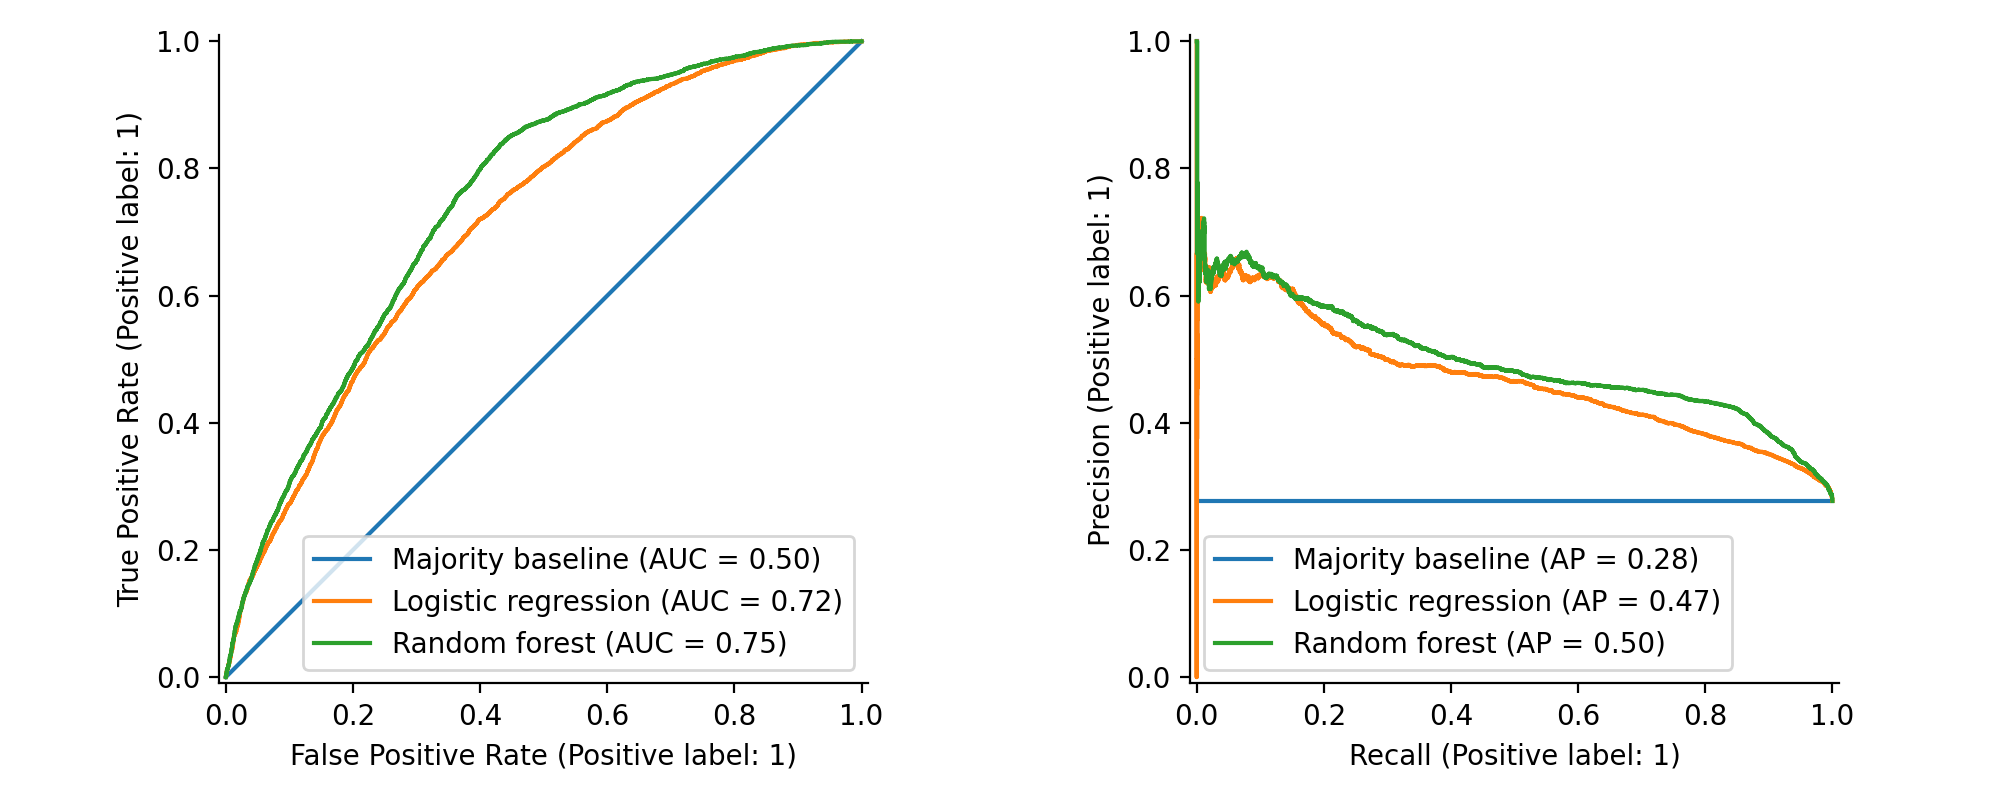
\includegraphics[width=\textwidth]{model_curves.png}
\caption{ROC and precision-recall curves for the final chronological test set. All models are predeclared; the curves do not revise validation-based selection.}\label{fig:curves}
\end{figure*}

\subsection{Generalization and Feature Interpretation}
Logistic regression's training ROC-AUC is 0.7948 and validation ROC-AUC is 0.7910, falling to 0.7180 on test. Average precision is 0.6024, 0.7031, and 0.4694, respectively. AP values are affected by differing class prevalence as well as ranking. The test decline is consistent with temporal distribution change and limited transportability; it does not establish a particular causal explanation.

The forest's training ROC-AUC is 0.8381, compared with 0.8253 on validation and 0.7501 on test. Restricted depth and minimum leaf size reduce excessive complexity, but do not guarantee absence of overfitting. Neither model should be treated as ready for unattended operational use. Multiple rolling origins, prospective snapshots, and calibration assessment are appropriate next steps.

Permutation importance is calculated on a fixed random validation sample of 3,500 bookings using three repeats and decrease in average precision. Lead time has the largest mean decrease, 0.2142, followed by market segment at 0.0746, country at 0.0352, and hotel at 0.0319. These rankings align with the main EDA comparisons. A negative importance, such as that observed for arrival month in this sample, means shuffling improved the measured score; it is not evidence that the feature causally protects a booking.

\begin{figure}[htbp]\centering
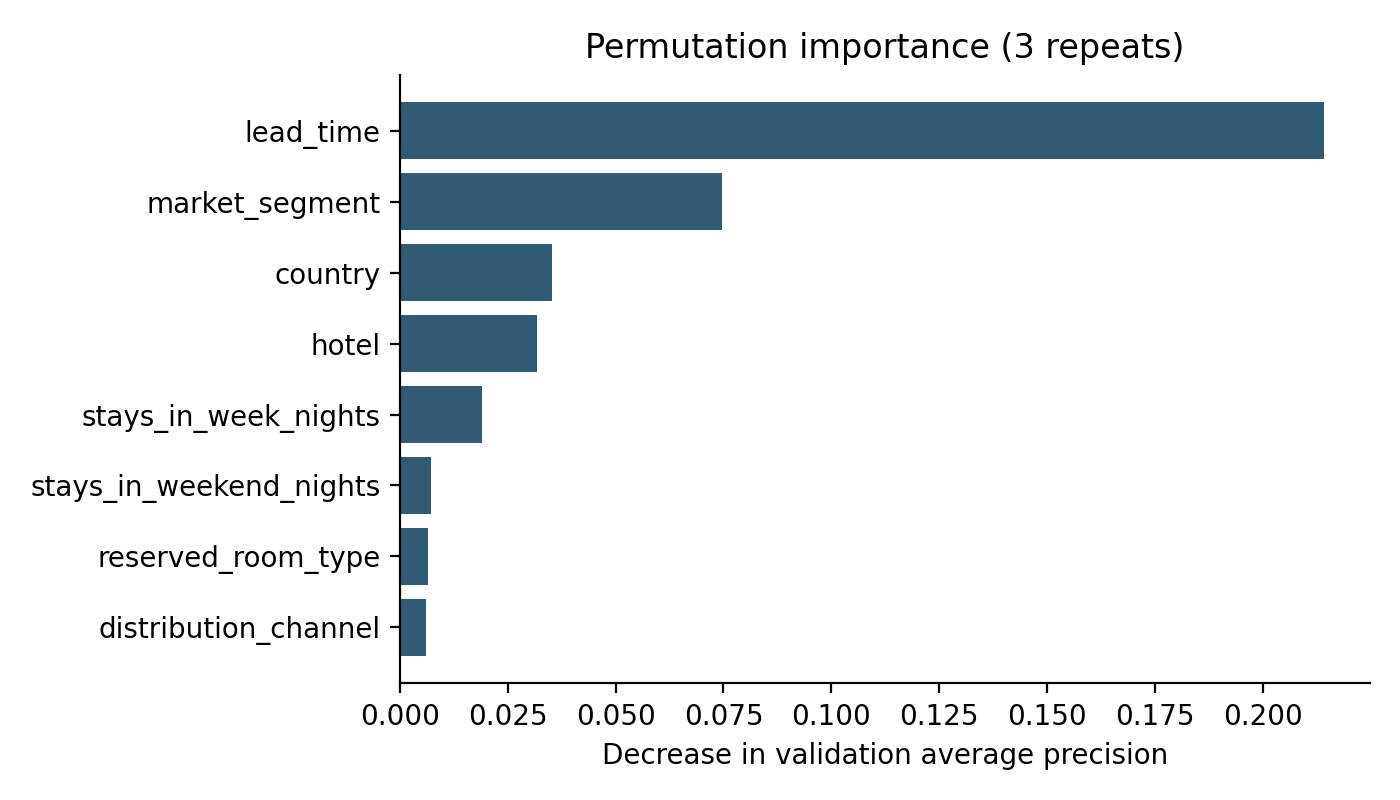
\includegraphics[width=\columnwidth]{importance.png}
\caption{Validation permutation importance of the selected logistic model. Values measure a predictive score change, not causal business effects.}\label{fig:importance}
\end{figure}

\subsection{Raw-Record Sensitivity}
Keeping all raw records and the same date boundaries, we retrain the selected model type without changing its settings. On the raw later test sample it reaches ROC-AUC 0.7355, average precision 0.5663, precision 0.6135, recall 0.3379, and F1 0.4357. This is a sensitivity analysis on a different row-weighting scheme, not an independent validation. It shows that repeated-record handling materially changes both prevalence and reported performance.

\section{Discussion and Recommendations}
\subsection{Capacity-Limited Follow-Up}
A manager may have capacity for a fixed number of confirmations rather than a universal probability cutoff. We therefore evaluate a predeclared highest-risk decile of the selected model's final-test scores. Rounding capacity upward gives 1,757 reservations. Of these, 977 historically canceled, yielding 55.61\% precision and capturing 20.08\% of all 4,865 test cancellations. Relative to 27.70\% test prevalence, this is 2.01-fold enrichment.

This result means that the historical queue concentrates cancellations; it does not mean 977 cancellations can be prevented. Approximately 780 queue bookings did not cancel, and most test cancellations remain outside the queue. Contact should therefore be supportive and inexpensive. Recommended actions include confirming arrival intent and booking details, offering policy-consistent modifications, and recording the guest's response. A high score alone should not trigger a penalty or automatic cancellation.

The application provides a 5--30\% workload slider, shows enrichment and cancellation capture for the selected cohort, and downloads a queue without revealing retrospective outcomes in the exported action list. Stable extract-level review references help distinguish rows; they are not actual reservation identifiers. Filters restrict queue membership to matching held-out bookings. This is a demonstration of historical prioritization, not a live integration with a property-management system. The 10\% reported study result remains fixed even though users can explore other capacities.

\subsection{Measuring Business Impact}
Before routine use, managers should randomize eligible high-risk bookings to confirmation and usual-care groups, with appropriate guest-service oversight. Compare cancellation rates, completed stays, contact costs, complaints, and operational workload. The primary endpoint and analysis period should be specified before observing the pilot outcomes. Randomization would help distinguish intervention effects from the fact that contacted bookings were initially riskier.

No currency savings are estimated here because intervention effectiveness, contact cost, occupancy recovery, and contribution margins are not supplied. If a pilot established incremental retained stays, a later calculation could combine that effect with verified margin and workload costs. Multiplying all canceled bookings by daily rate would overstate supported evidence and ignore whether rooms were resold.

\subsection{Limitations and Responsible Use}
The two-property, historical sample cannot establish current performance at other hotels. Arrival-window truncation and incomplete boundary years distort naive seasonality and creation-date cohort interpretation. Purging unresolved labels improves time consistency but may emphasize reservations that resolve sooner. Exact-row removal is contestable without unique reservation identifiers, and the sensitivity results show why this choice matters.

Candidate inputs need a booking-time availability audit. Country, channel, and customer-type features can also create uneven errors across groups. The prototype reports overall metrics; subgroup calibration and error comparisons remain future work. Staff should review reservations according to consistent service standards and should not infer personal intent from a risk score.

The app is tested for basic interactions, not employee adoption or long-term operational reliability. There is no automatic retraining, persistent user database, authentication layer, or production integration. These omissions are consistent with a local educational prototype. For later deployment, add versioned snapshots, validation checks, monitored drift, access control, and a documented escalation path for incorrect predictions.

\section{Conclusion and Future Work}
This project connects a descriptive hotel-booking dashboard with a reproducible chronological classification study. The dashboard makes cancellation exposure comparable across properties, segments, arrival periods, and lead-time groups, while preserving group counts and interpretation notes. Logistic regression, selected using validation average precision, provides useful but limited discrimination on later bookings. Its top-decile queue doubles the observed concentration of cancellations relative to test prevalence, while missing most cancellations and identifying many reservations that ultimately remain active.

The practical recommendation is a monitored confirmation pilot rather than automatic enforcement or a claim of realized savings. Future work should collect complete booking-created cohorts, preserve event histories, resolve duplicate identity, compare rolling temporal validation windows, audit subgroup errors, and measure intervention effects prospectively. The locally executable code, notebook, CSVs, and exported results provide a transparent basis for that extension.

\begin{thebibliography}{00}
\bibitem{dataset} N. Antonio, A. de Almeida, and L. Nunes, ``Hotel booking demand datasets,'' \emph{Data in Brief}, vol. 22, pp. 41--49, 2019, doi: 10.1016/j.dib.2018.11.126.
\bibitem{hotelprediction} N. Antonio, A. de Almeida, and L. Nunes, ``Predicting hotel booking cancellations to decrease uncertainty and increase revenue,'' \emph{Tourism \& Management Studies}, vol. 13, no. 2, pp. 25--39, 2017, doi: 10.18089/tms.2017.13203.
\bibitem{breiman} L. Breiman, ``Random forests,'' \emph{Machine Learning}, vol. 45, pp. 5--32, 2001, doi: 10.1023/A:1010933404324.
\bibitem{sklearn} F. Pedregosa et al., ``Scikit-learn: Machine learning in Python,'' \emph{Journal of Machine Learning Research}, vol. 12, pp. 2825--2830, 2011.
\bibitem{pitfalls} Scikit-learn developers, ``Common pitfalls and recommended practices.'' Accessed: Nov. 4, 2026. [Online]. Available: \url{https://scikit-learn.org/stable/common_pitfalls.html}
\bibitem{saito} T. Saito and M. Rehmsmeier, ``The precision-recall plot is more informative than the ROC plot when evaluating binary classifiers on imbalanced datasets,'' \emph{PLOS ONE}, vol. 10, no. 3, Art. no. e0118432, 2015, doi: 10.1371/journal.pone.0118432.
\bibitem{metrics} Scikit-learn developers, ``Metrics and scoring: Quantifying the quality of predictions.'' Accessed: Nov. 4, 2026. [Online]. Available: \url{https://scikit-learn.org/stable/modules/model_evaluation.html}
\end{thebibliography}
\end{document}
